\section{Problem set 1}

\subsection{Problem 1}
  Let \( A(a_{1},a_{2}) \), \( B(b_{1},b_{2}) \) be two points in \( \mathbb{R}^{2} \). Find
  the equation for the line \( \ell(A,B) \) through \( A \), \( B \).
  \begin{enumerate}
    \item in Cartesian form.
    \item in parametric vector form.
  \end{enumerate}

\begin{solution}
 Cartesian form:
 For all \( \left(x,y  \right) \in l \) 
 \begin{align*}
    \frac{b_{2}-a_{2}}{b_{1}-a_{1}} &= \frac{y-a_{2}}{x-a_{1}} \\
    \left( x-a_{1} \right) \left( b_{2}-a_{2} \right) &= \left( y-a_{2} \right) \left( b_{1} - a_{1} \right)     \\
    xb_{2} - xa_{2} - a_{1}b_{1} + a_{1}a_{2} &= yb_{1} - ya_{1} -a_{2}b_{2} + a_{1}a_{2} \\
    x(b_{2}-a_{2}) - a_{1}b_{2} + a_{2}b_{1} &= y \left( b_{1}-a_{1} \right) \\
                                             y &= \frac{x \left( b_{2}-a_{1} \right)}{b_{1}-a_{1}} + \frac{-a_{1}b_{2}+b_{2}b_{1}}{b_{1}-b_{1}} 
  .\end{align*}
 \end{solution}

 So, above is the cartesian equation of \( \ell \). \\
 
 Parametric form: \( A = \begin{pmatrix} a_{1} \\ a_{1} \end{pmatrix}, B = \begin{pmatrix} b_{1} \\ b_{2} \end{pmatrix}  \). We treat
\( A \) and \( B \) as position veectors. Then,
\[
  \overrightarrow{AB} = \begin{pmatrix} b_{1}-a_{1} \\b_{2}-a_{2} \end{pmatrix} 
.\] 
is parallel to \( \ell \). Hence the parametric form is, for all \( \begin{pmatrix} x \\ y \end{pmatrix} \in \ell \),

\[
  \begin{pmatrix} x \\ y \end{pmatrix}  = \begin{pmatrix} a_{1}\\a_{1} \end{pmatrix}  + \lambda \begin{pmatrix} b_{1}-a_{1}\\b_{2}-a_{2} \end{pmatrix}
.\]
for some \( \lambda \in \mathbb{R} \). (Ask lect best way to write eqn)

\subsection{Problem 2}

For any vectors \( \mathbf{a}, \mathbf{b}, \mathbf{c} \in \mathbb{R}^{n}   \) and scalar \( \lambda \in \mathbb{R} \),
\begin{enumerate}
  \item \( \mathbf{a} \cdot \mathbf{b} \in \mathbb{R} \) (Scalar).
  \item \( \mathbf{a} \cdot \mathbf{a} = |\mathbf{a} |^{2} \), \( |\mathbf{a} | = \sqrt{\mathbf{a}\cdot \mathbf{a}} \).
  \item \( \mathbf{a} \cdot \mathbf{b} = \mathbf{b} \cdot \mathbf{a} \), (commutativity)
  \item \( \mathbf{a} \cdot (\lambda \mathbf{b}) = \lambda \left( \mathbf{a} \cdot \mathbf{b} \right)  \)
  \item \( \mathbf{a} \cdot \left( \mathbf{b} + \mathbf{c} \right) = \mathbf{a} \cdot \mathbf{b} + \mathbf{a} \cdot \mathbf{c} \), (distributive)
  \item If \( \mathbf{a}, \mathbf{a} \in  \mathbb{R}^{n}\) then \( |\mathbf{a} \cdot \mathbf{b}| \le | \mathbf{a} | |\mathbf{b} |\)  (cauchy-schwarz Inequality)
  \item Hence, the angle \( \theta  \) between \( \mathbf{a}, \mathbf{b} \) via \( \cos \theta  = \frac{\mathbf{a}\cdot \mathbf{b}}{| \mathbf{a}| |\mathbf{b} |} \) is well defined.
  \item For \( \mathbf{a}, \mathbf{b} \in \mathbb{R}^{n}, |\mathbf{a} + \mathbf{b} | \le |\mathbf{a} | + \mathbf{b}\)  (Triangle inequality).
  \item Use the dot product to prove that a real \( n \times n  \) matrix \( Q \) is an orthogonal matrix
    if and only if \( Q \mathbf{x} \cdot Q\mathbf{x} = \mathbf{x} \cdot \mathbf{x}  \) for all \( \mathbf{x} \in \mathbb{R}^{n} \).
\end{enumerate}

\begin{solution}
We first prove \( Q \mathbf{x} \cdot Q\mathbf{x} = \mathbf{x} \cdot \mathbf{x}, \; \forall \mathbf{x} \in \mathbb{R}^{n} \implies Q \)  is orthogonal.
\begin{align*}
  Q \mathbf{x} \cdot Q \mathbf{x} &= \mathbf{x} \cdot \mathbf{x} \\
  (Q \mathbf{x} \cdot Q \mathbf{x}) &= (\mathbf{x} \cdot \mathbf{x}) \\
  (Q \mathbf{x})^{T} Q \mathbf{x} &= \mathbf{x}^{T} \mathbf{x}  \\ 
  \mathbf{x}^{T} Q^{T}Q \mathbf{x} &= \mathbf{x}^{T} \mathbf{x}
.\end{align*}
left multiplying \( \left( \mathbf{x}^{T} \right)^{-1} \) on both sides and
right multiplying  \( \left( \mathbf{x} \right)^{-1} \) on both sides we get,
\[
  Q^{T}Q = I
.\] 

Note that the algebra above is reversible therefore the converse is also true.
\end{solution}

\subsection{Problem 3}
Consider the points \( A(\mathbf{a}), B \left( \mathbf{b} \right) \) and the origina \( O \) and \( \triangle OAB \) and let \( \theta = \angle AOB \). Use 
the Cosine Law to deduce \( \cos  \theta = \frac{\mathbf{a} \cdot \mathbf{b}}{|\mathbf{a} | |\mathbf{b} |}  \).

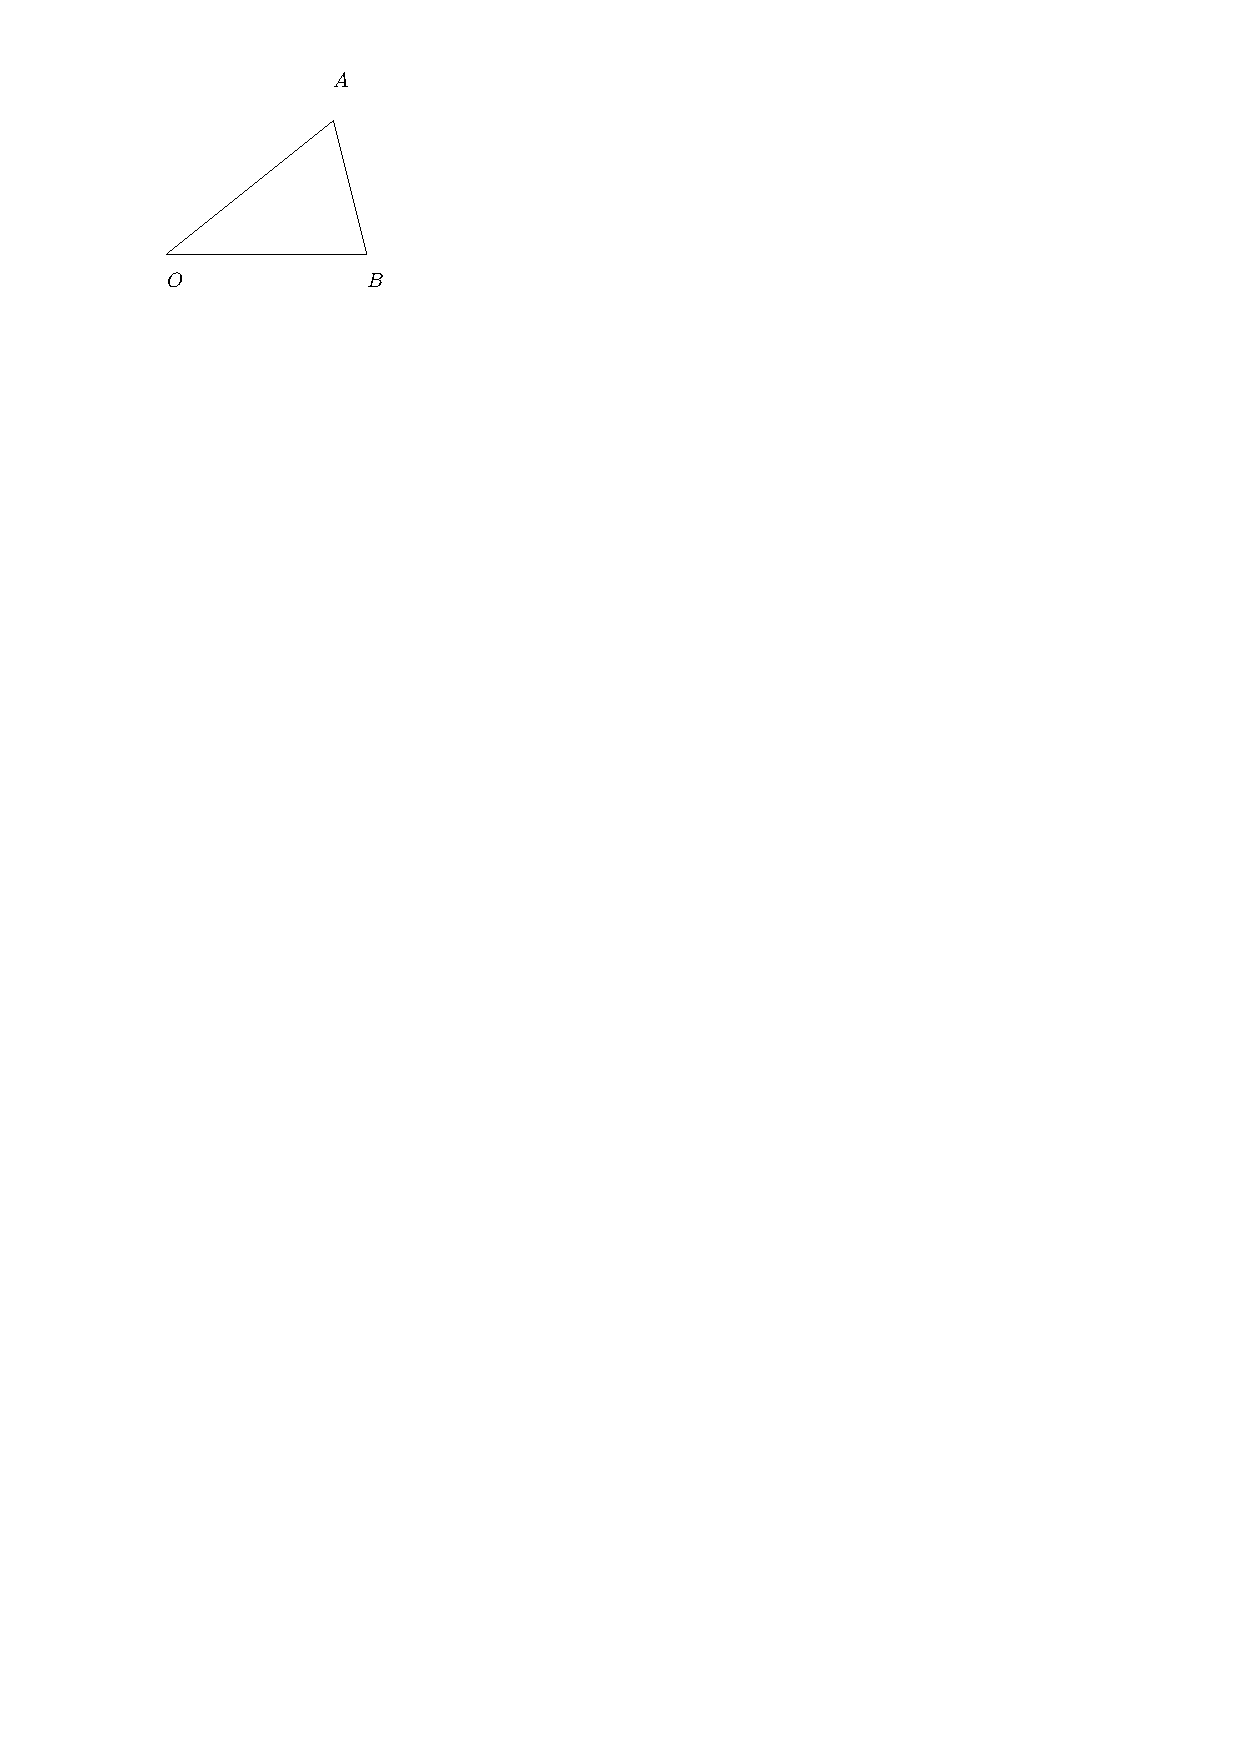
\includegraphics{./figures/fig1}

\begin{solution}


  Using the cosine rule we get, 
  \begin{align*}
    | \mathbf{a} - \mathbf{b} |^{2} &= | \mathbf{a} |^{2} + | \mathbf{b} |^{2} - 2 | \mathbf{a} | | \mathbf{b} | \cos \theta  \\
    2 | \mathbf{a} | | \mathbf{b} | \cos  \theta &= | \mathbf{a} |^{2} + | \mathbf{b} |^{2} - | \mathbf{a} - \mathbf{b} |^{2}     \\
    \cos  \theta  &= \frac{| \mathbf{a} |^{2} = | \mathbf{b} |^{2} - | \mathbf{a} - \mathbf{b} |^{2} }{2 | \mathbf{a} | | \mathbf{b} |} \\
                  \cos  \theta  &= \frac{\mathbf{a} \cdot \mathbf{a} + \mathbf{b} \cdot \mathbf{b} - \left( \mathbf{a - \mathbf{b}} \right) \cdot \left( \mathbf{a} - \mathbf{b} \right)}{2 | \mathbf{a} | | \mathbf{b} |} \\
                  &=   \frac{2\mathbf{b} \cdot \mathbf{a}}{2 | \mathbf{a} | | \mathbf{b} |} \\
                  &= \frac{\mathbf{a} \cdot \mathbf{b}}{| \mathbf{a} | | \mathbf{b} |}
.\end{align*}

\end{solution}

\subsection{Problem 4}

Show that a collineation determines a 1-1 correspondence from the set of all lines to itself.

\begin{solution}
  Clarify meaning of question.
\end{solution}

\subsection{Problem 5}

Show that the lines with equations \( aX + bY + c = 0 \) and \( dX + eY + f = 0 \) are parallel iff \( ae - bd = 0 \) and 
are perpendicular iff \( ad + be = 0 \).

\begin{solution}
  We first rewrite the equations in the form \( Y = mX + b \).
  We get \( Y = -\frac{a}{b}X - \frac{c}{b} \) and \( Y  = -\frac{d}{c} - \frac{c}{e}\)
  We know these lines are parellel if,
  \begin{align*}
    -\frac{a}{b} &= -\frac{d}{e} \\
    -ae &= -db \\
    ae - db &= 0
  .\end{align*}
  Therefore, backwards implication proved. Forward implication is just obtained 
  with the same algebra above since we can assume that the lines are parallel and gradients are equal once again giving us \( ae - db = 0 \).

  Now we prove the condition for perpendicular lines. We know these lines
  are perpendicular if,

  \begin{align*}
    \frac{b}{a} &= -\frac{d}{e} \\
  ad + be &= 0 
  .\end{align*}
  Hence, backward implication proved. Forward implication
  once again proved by same algebra above through similar reasoning with
  forward implication of parallel lines.
\end{solution}

\subsection{Problem 6}
A multiplication for finite gorup is often called Cayley table. Find the cayley table for the group \( V_{4} = \{1, \sigma , \alpha , \beta \}  \) which
is defined by the transformations
\[
  1 \left( x,y \right) = \left( x,y \right), \sigma \left( x, y \right) = \left( -x, -y \right), \alpha \left(x, y  \right) = \left(x, -y  \right), \beta \left( x,y \right) = \left( -x,y \right)
.\] 
For all \( \left( x,y \right) \in \mathbb{R}^{2} \).

\begin{solution}

  \begin{tabular}{ c c c c c }
    \( V_{4} \) & 1 & \( \sigma  \) & \( \alpha  \) & \( \beta  \) \\
    1 & 1 & \( \sigma  \) & \( \alpha  \) & \( \beta  \) \\
  \( \sigma  \) & \( \sigma  \) & 1 & \( \beta  \) & \( \alpha  \) \\
  \( \alpha  \) & \( \alpha   \) & \( \beta   \) & \(1  \) & \( \sigma  \) \\
  \( \beta  \) & \( \beta  \) & \( \alpha   \)& \( \sigma  \) & 1
   
  \end{tabular}

\end{solution}

\subsection{Problem 7}

Suppose \( A,B,C \) are non collinear points. Then \( \tau_{A,B} = \tau_{C,D} \) \( \iff \square ABCD\)  is a parellelogram.

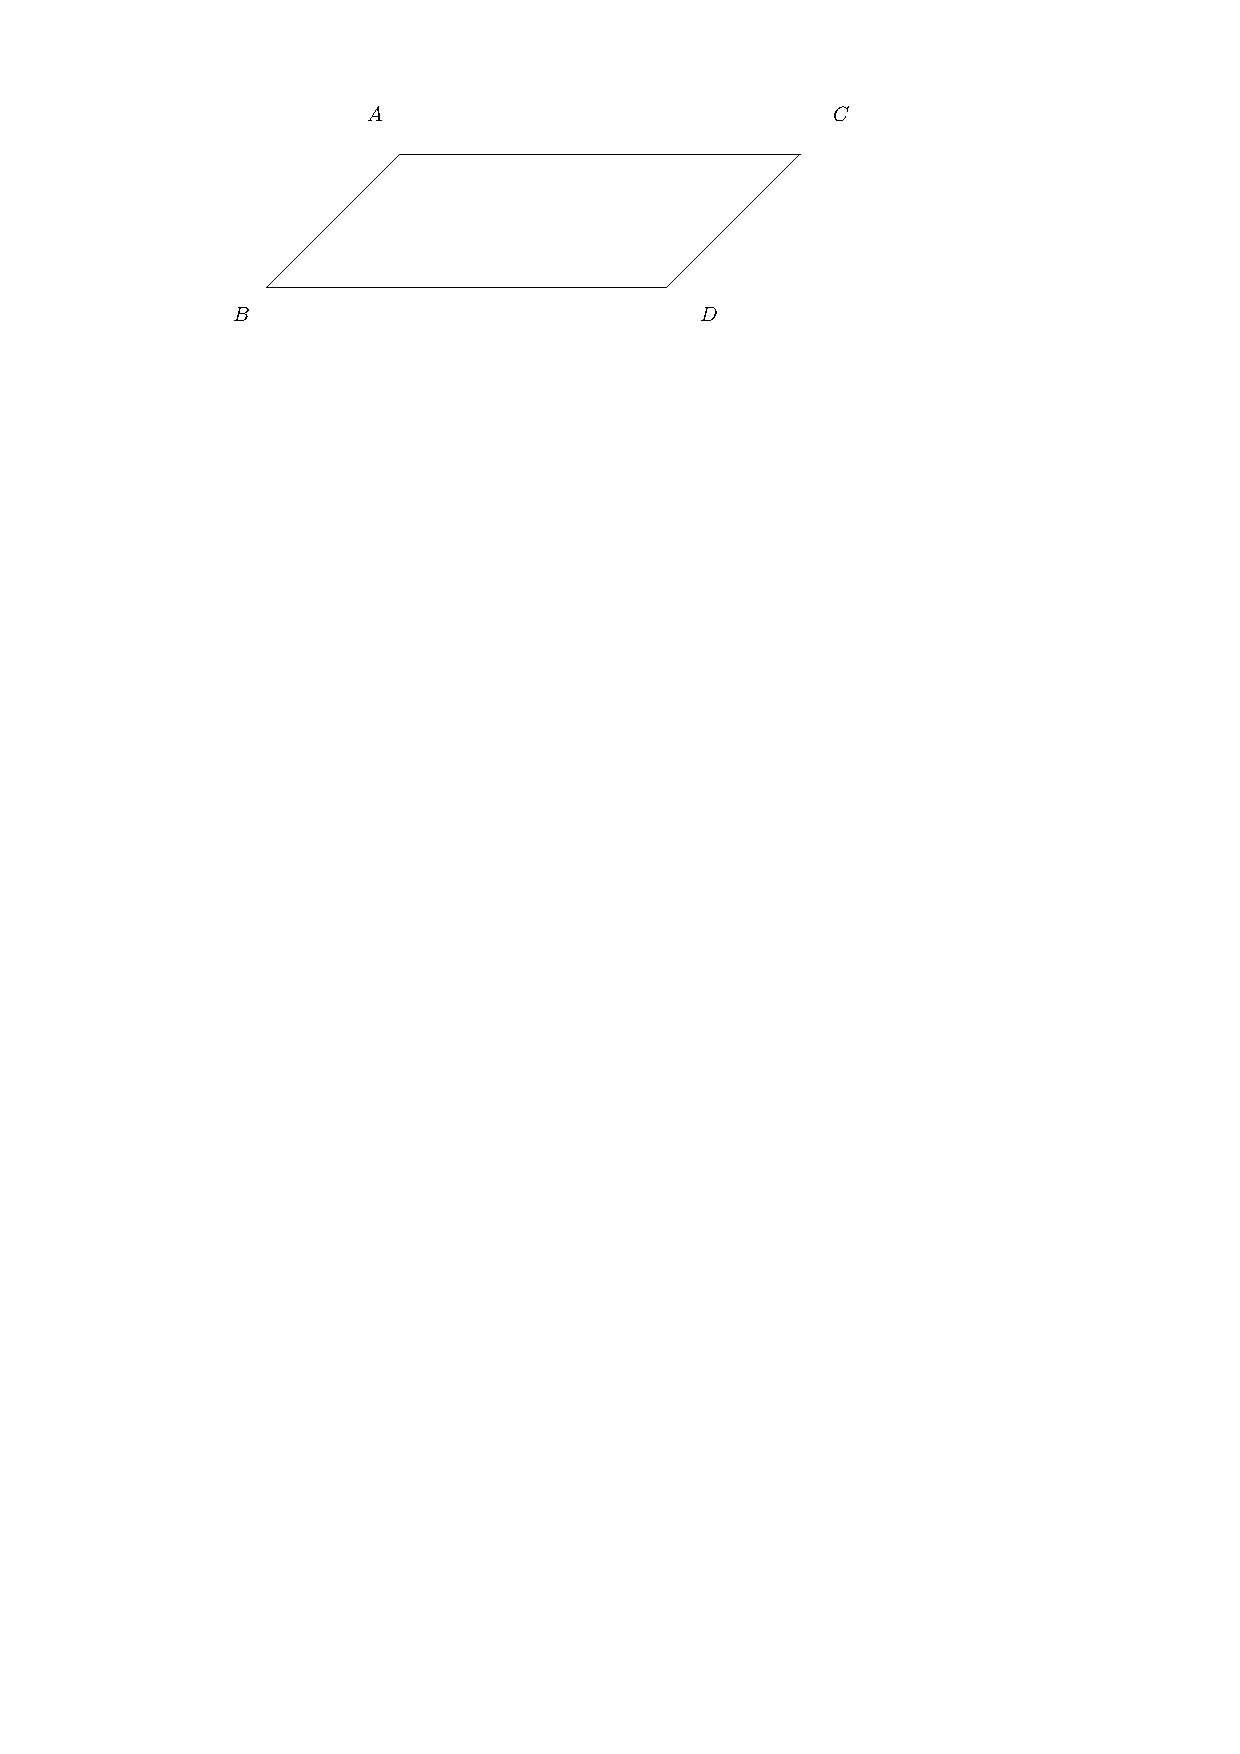
\includegraphics{./figures/q7Plgm.pdf}

\begin{solution}
  We show forward implication first.
  \[
    \tau_{A,B} = \tau_{C,D} \implies \overrightarrow{AB} = \overrightarrow{CD}
  .\] 

  So, \( | \overrightarrow{AB} | = |  \overrightarrow{CD} | \) and \( AB \parallel CD \).
  Now, it remains to show \( AB \) and \( CD \) do not lie on the same line.
  We know that \( A,B,C \) are non collinear. We show that \( A,B,D \) are non collinear.
 Assume that \( A,B,D  \) are collinear, then \( A, D, C \) are non collinear and form a triangle. Then \( CD \) intersects \( AD \)
 and hence  \( \ell(AB) \) as \( B \) lies on \( \ell(AD) \). If \( CD \) intersects \( \ell(AB) \) then \( AB \) and \( CD \)
 cannot be parallel which is a contradiction as we have already proven them to be parallel.
 Therefore our assumption that \( A,B,D \) are collinear is false. So, \( A,B,C \) are non collinear and \( A,B,D \)
 are non collinear. Hence \( CD \) does not lie \( \ell(AB) \). Therefore \( AB \) and \( CD \) are congruent and parallel sides 
 of a parallelogram \( CABD \).

 Backward implication follows immediately from the congruence of \( AB \) and \( CD \) and therefore their vectors being equal 
 as they are two sides of a parallelogram. Giving is the equality of the isometry.

 \end{solution}
